\documentclass[11pt,a4paper]{article}


\usepackage{tabularx}
\usepackage[latin1]{inputenc}
\usepackage{fullpage}
\usepackage{amsmath}
\usepackage{amssymb}
\usepackage{enumerate}
\usepackage{xcolor}
\usepackage{tikz}

\def\layersep{2.5cm}

\title{Leren --- Homework 5\\[3mm]\small{Chapter 11, Alpaydin}}
\date{Deadline: 23:59 December 16th, 2018}

\newcommand{\ab}{\mathbf{a}}
\newcommand{\xb}{\mathbf{x}}
\newcommand{\vb}{\mathbf{v}}
\newcommand{\wb}{\mathbf{w}}
\newcommand{\hb}{\mathbf{h}}
\newcommand{\sbold}{\mathbf{s}}
\newcommand{\Wb}{\mathbf{W}}
\newcommand{\Xb}{\mathbf{X}}
\newcommand{\lp}{\left(}
\newcommand{\rp}{\right)}

\begin{document}

\maketitle

\noindent Artificial neural networks are machine learning models. These models can be trained with \textit{gradient descent}: small steps in the direction of the gradient are taken, to minimize/maximize a loss/likelihood function. Therefore, to train a model, we need two things: how to compute the prediction (forward), and how to compute the gradient (backward).



\section{Multinomial Regression / Multiclass Discrimination}

\begin{figure}[h]
\centering
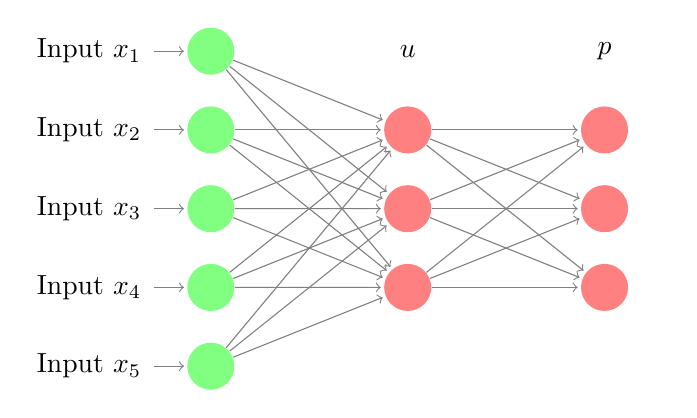
\begin{tikzpicture}[shorten >=1pt,->,draw=black!50, node distance=\layersep]
    \tikzstyle{every pin edge}=[<-,shorten <=1pt]
    \tikzstyle{neuron}=[circle,fill=black!25,minimum size=17pt,inner sep=0pt]
    \tikzstyle{input neuron}=[neuron, fill=green!50];
    \tikzstyle{output neuron}=[neuron, fill=red!50];
    \tikzstyle{hidden neuron}=[neuron, fill=blue!50];
    \tikzstyle{annot} = [text width=4em, text centered]

    % Draw the input layer nodes
    \foreach \name / \y in {1,...,5}
    % This is the same as writing \foreach \name / \y in {1/1,2/2,3/3,4/4}
        \node[input neuron, pin=left:Input $x_\y$] (I-\name) at (0,-\y) {};

    % Draw the hidden layer nodes
    \foreach \name / \y in {1,...,3}
        \path[yshift=-1cm]
            node[output neuron] (U-\name) at (\layersep,-\y cm) {};
            % node[hidden neuron,pin={[pin edge={->}]}] (U-\name) at (\layersep,-\y cm) {};

    \foreach \name / \y in {1,...,3}
        \path[yshift=-1cm]
            node[output neuron] (P-\name) at (5cm,-\y cm) {};

    % Connect every node in the input layer with every node in the
    % hidden layer.
    \foreach \source in {1,...,5}
        \foreach \dest in {1,...,3}
            \path (I-\source) edge (U-\dest);

    \foreach \source in {1,...,3}
        \foreach \dest in {1,...,3}
            \path (U-\source) edge (P-\dest);
    

    \node[annot,above of=U-1, node distance=1cm] (hl) {$u$};
    \node[annot,above of=P-1, node distance=1cm] (hl) {$p$};

\end{tikzpicture}
\caption{Multinomial Regression}
\end{figure}

\noindent Multinomial regression models make predictions for multi-class problems. The likelihood for such a classification problem, given a dataset $\{(\xb^{(i)}, t^{(i)})\}_{i=1}^N$, is written as:
\[ \prod_{i=1}^N p(t^{(i)} | \xb^{(i)})\]

\noindent And the log-likelihood as:
\[ \mathcal{L} = \sum_{i=1}^N \log p(t^{(i)} | \xb^{(i)})\]

\noindent For now, we will focus on the likelihood of a single datapoint and omit the $^{(i)}$ notation. Also we let $p(t | \xb) = p_t$:
\[ \ell = \log p(t | \xb) = \log p_t\]


\noindent For every class $j = 1, \ldots, C$, a value $u_j$ is put through a softmax to obtain
a probability distribution over classes. The probability that $\xb$ belongs to class $j$, $p_j = p(j | \xb)$, is defined as:

\[ p_j = \frac{\exp(u_j)}{\sum_{k=1}^C \exp(u_k)} \]
this ensures that the sum of probabilities $\sum_j p_j$ is equal to $1$. \\

And we can write $\log p_j$ as:
\[ \log p_j = u_j - \log {\sum_{k=1}^C \exp u_k} \]

\noindent In this first part we choose a simple linear model for $u_j$. In this equation $\wb_j$ and $b_j$ are parameters.:


\[ u_j(\xb) = \wb_j^T\xb + b_j \] 



\noindent These equations together define the prediction/forward computation of the multinomial regression model. To optimize the likelihood, we will use a gradient method. As such, gradients from the likelihood to the parameters are needed: $\frac{\partial \mathcal{\ell}}{\partial \wb_j}$ and $\frac{\partial \ell}{\partial b_j}$, for all $j$. To obtain these, we use the chain rule and find expressions for $\frac{\partial \mathcal{\ell}}{\partial u_j}$, $\frac{\partial u_j}{\partial \wb_j}$ and $\frac{\partial u_j}{\partial b_j}$.

\begin{enumerate}[(a)]
\item Show that $\frac{\partial \ell}{\partial u_j}$ is equal to $\left.
  \begin{cases}
    1 - \frac{\exp u_j}{\sum_{k=1}^C \exp u_k}, & \text{if } j = t \\
    \text{   }- \frac{\exp u_j}{\sum_{k=1}^C \exp u_k}, & \text{if } j \not= t \\
  \end{cases}
  \right\}$
\item Give the derivative for $\frac{\partial u_j}{\partial \wb_j}$
\item Give the derivative for $\frac{\partial u_j}{\partial b_j}$
\item Give an expression for the gradient $\frac{\partial \ell}{\partial \wb_j}$ and $\frac{\partial \ell}{\partial b_j}$
\item Explain why the derivative $\frac{\partial u_j}{\partial \wb_i}$ is 0, if $i \not= j$.
\end{enumerate}


\section{Neural Networks}

\begin{figure}[h]
\centering
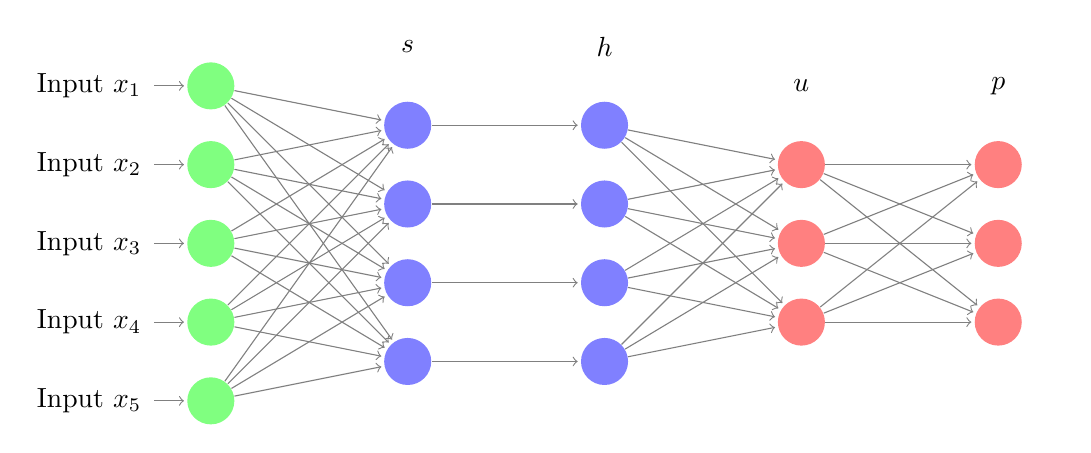
\begin{tikzpicture}[shorten >=1pt,->,draw=black!50, node distance=\layersep]
    \tikzstyle{every pin edge}=[<-,shorten <=1pt]
    \tikzstyle{neuron}=[circle,fill=black!25,minimum size=17pt,inner sep=0pt]
    \tikzstyle{input neuron}=[neuron, fill=green!50];
    \tikzstyle{output neuron}=[neuron, fill=red!50];
    \tikzstyle{hidden neuron}=[neuron, fill=blue!50];
    \tikzstyle{annot} = [text width=4em, text centered]

    % Draw the input layer nodes
    \foreach \name / \y in {1,...,5}
    % This is the same as writing \foreach \name / \y in {1/1,2/2,3/3,4/4}
        \node[input neuron, pin=left:Input $x_\y$] (I-\name) at (0,-\y) {};

    % Draw the hidden layer nodes
    \foreach \name / \y in {1,...,4}
        \path[yshift=-.5cm]
            node[hidden neuron] (S-\name) at (\layersep,-\y cm) {};
            % node[hidden neuron,pin={[pin edge={->}]}] (U-\name) at (\layersep,-\y cm) {};

        % Draw the hidden layer nodes
    \foreach \name / \y in {1,...,4}
        \path[yshift=-.5cm]
            node[hidden neuron] (H-\name) at (5cm,-\y cm) {};
            % node[hidden neuron,pin={[pin edge={->}]}] (U-\name) at (\layersep,-\y cm) {};

    % Draw the hidden layer nodes
    \foreach \name / \y in {1,...,3}
        \path[yshift=-1cm]
            node[output neuron] (U-\name) at (7.5cm,-\y cm) {};
            % node[hidden neuron,pin={[pin edge={->}]}] (U-\name) at (\layersep,-\y cm) {};

    \foreach \name / \y in {1,...,3}
        \path[yshift=-1cm]
            node[output neuron] (P-\name) at (10cm,-\y cm) {};

    % Connect every node in the input layer with every node in the
    % hidden layer.
    \foreach \source in {1,...,5}
        \foreach \dest in {1,...,4}
            \path (I-\source) edge (S-\dest);

    \foreach \y in {1,...,4}
        \path (S-\y) edge (H-\y);

    \foreach \source in {1,...,4}
        \foreach \dest in {1,...,3}
            \path (H-\source) edge (U-\dest);

    \foreach \source in {1,...,3}
        \foreach \dest in {1,...,3}
            \path (U-\source) edge (P-\dest);
    
    \node[annot,above of=S-1, node distance=1cm] (hl) {$s$};
    \node[annot,above of=H-1, node distance=1cm] (hl) {$h$};
    \node[annot,above of=U-1, node distance=1cm] (hl) {$u$};
    \node[annot,above of=P-1, node distance=1cm] (hl) {$p$};

\end{tikzpicture}
\caption{Neural Network}
\end{figure}


\noindent In the previous exercise, the unnormalized probability $u_j$ was a linear model of $\xb$. In neural networks, multiple linear models can be stacked and alternated with activations functions:

We let $u_j$ be a linear function of hidden layer $\hb$.
\[ u_j = \wb_j^T \hb + b_j \]

\noindent The hidden layer $\hb$ is obtained by applying a sigmoid activation function on the pre-activations $\sbold$.
\[ h_k = \sigma(s_k) = \frac{1}{1 + \exp(-s_k)} \]

And the pre-activations $\sbold$ are a linear function of $\xb$.
\[ s_k = \vb_k^T \xb + a_k \]



\begin{enumerate}[(a)]
\item Give an expression for $\frac{\partial \ell}{\partial \wb}$ and $\frac{\partial \ell}{\partial b_j}$. (Hint: Answer is similar to the previous exercise)
\item Derive $\frac{\partial \ell}{\partial h_k}$ and show it is equal to $\sum_j \frac{\partial \ell}{\partial u_j} w_{jk}$. (Hint: use $\frac{\partial \ell}{\partial h_k} = \sum_j \frac{\partial \ell}{\partial u_j}\frac{\partial u_j}{\partial h_k}$)
\item Derive $\frac{\partial h_k}{\partial s_k}$ and show it is equal to $h_k (1 - h_k)$.
\item Derive $\frac{\partial s_k}{\partial \vb_k}$ and $\frac{\partial s_k}{\partial a_k}$
\item Give the expression for the gradients $\frac{\partial \ell}{\partial \vb_k}$ and $\frac{\partial \ell}{\partial a_k}$
\end{enumerate}



\section{Open questions}
\begin{enumerate}[(a)]
\item Explain why we need gradients for in neural networks. And why do we not simply set the gradient of the likelihood to zero? 

\item Imagine we have a neural network with $k$ layers without non-linearities: $y(\xb) = \Wb_k \ldots \Wb_2 \Wb_1 \xb $. Show or explain that this network cannot learn non-linear functions. 

\item What is an advantage of using mini-batches during the training of a neural network?
\end{enumerate}


\end{document}
